		The given line
parameters are
\begin{align}
		\vec{n} = \myvec{3\\2},\, c=12 ,\,
	\vec{m} =\myvec{-2 \\ 3}.
\end{align}
and the point on the y-axis is
\begin{align}
	\vec{A} =\myvec{0\\6}.
\end{align}
Thus, the equation of the desired line is 
\begin{align}
	\vec{m}^\top\brak{\vec{x}-\vec{A}}&=0\label{eq:chapters/11/10/4/7/5}
	\\
\implies
			\myvec{-2 & 3}\vec{x} &=-18
		\end{align}
		\iffalse
		See 
  \figref{fig:chapters/11/10/4/7/Figure}.
\begin{figure}[H]
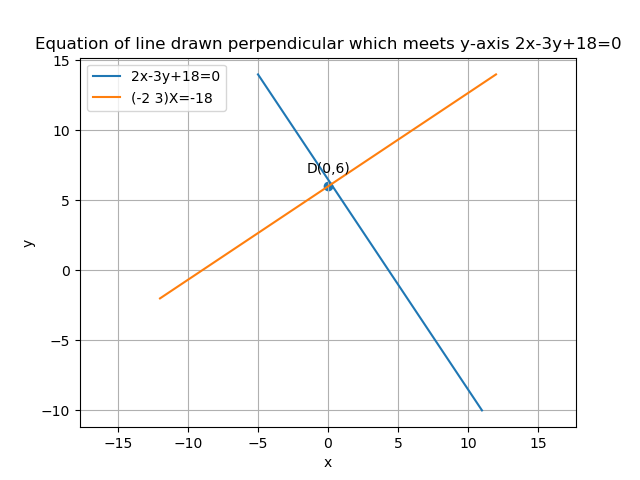
\includegraphics[width=0.75\columnwidth]{chapters/11/10/4/7/figs/fig.png}
\caption{}
  \label{fig:chapters/11/10/4/7/Figure}
\end{figure}
\fi
